\documentclass[12pt,a4paper]{article}
\usepackage{mathsx,tech,mytheorems}
\usepackage{tikz}
\usetikzlibrary{arrows}
\usepackage{scalalistings}%\unScalaMid

\newtheorem{lemma}{Lemma}
\newtheorem{prop}{Proposition}
\newtheorem{conjecture}[lemma]{Conjecture}
\newtheorem{definition}[lemma]{Definition}
\newtheorem{example}[lemma]{Example}
\newtheorem{assumption}[lemma]{Assumption}

\newtheorem{improve}{IMPROVE}
\newtheorem{impNote}{Implementation note}
\newtheorem{opt}{Optimisation}

\def\vec#1{\mathsf{#1}}
\def\trans#1{\stackrel{#1}\rightarrow}
\def\sqge{\sqsupseteq}
\def\sqle{\sqsubseteq}

\def\id{\mathrm{id}}
\def\params{\mathrm{params}}
%\def\srv{\vec{srvs}}
\def\fixed{\mathrm{fixed}}
\def\cpt{\mathrm{cpts}}
\def\cpts{\cpt}
\def\princ{\mathrm{princ}}
\def\S{\mathcal{S}}
\def\V{\mathcal{V}}

\def\mit{\it}

%\def\improve#1{IMPROVE: \emph{#1}}
%\def\impNote#1{\textbf{Implementation note:} #1}

%\def\floatpagefraction{0.85} 
\def\topfraction{0.9}

\everymath{\it}
\sloppy

\title{Improved View Abstraction: Working Paper}
\author{Gavin Lowe}

\begin{document}
\maketitle



\section{Setting}

Assume a state machine for each individual process. 

Each process state is a pair $(cs, ps)$ where $cs$~is a control state and $ps$
is a vector of parameters.  The first parameter of a component is always its
own identity.  Other parameters are references to other components.  For the
fixed process, all parameters are references to components.  Write $p.cs$ and
$p.\params$ for the control state and parameters of process state~$p$.  If $p$
is a component state, write $p.\id$ for its identity.
  
%%  We say that $s$ \emph{references} $id'$ if $id'$ is a parameter of~$s$
%% other than its own identity.

Write a system state as $s = (\fixed, \cpt)$ where $\fixed$ is the state of
the fixed process, and $\cpt$ is a set of states of components.  Write $\S$
for the set of all system states.  Write $s.\fixed$ and $s.\cpt$ for the fixed
processes or components, respectively.

If $s$ is a system state and $cpts$ is a set of component states with identities
disjoint from $s.\cpt$, then write $s \uplus cpts$ for $(s.\fixed, s.\cpt \union
cpts)$.  If $cpt$ is a component state, we abuse notation and write $cpt \in
s$ for $cpt \in s.\cpt$.

Assume different components have different identities for now. 

%% If $id$ is an identity, we say that $id$ is in $s$ if there is a
%% component~$cpt \in s$ such that $s.\id = id$.  We say that $s$ references $id$
%% if a component of~$s$ references~$id$. 

Assume that components are partitioned into \emph{active} and \emph{passive}
components.  E.g.~threads and nodes.  Each transition involves precisely one
active component or an active fixed process. 

\improve{check this in implementation.}


\section{View abstraction}

Define views as substates.
\begin{eqnarray*}
(\fixed, \cpt ) \sqle (\fixed', \cpt') & iff & 
  \fixed = \fixed' \land \cpt \subseteq \cpt' .
\end{eqnarray*}

%% Assume $\S$ is downwards-closed under taking substates. 

Fix a set $\V \subseteq \S$ of views.

Given a system state $s$, let
%
\begin{eqnarray*}
\alpha(s) & = &
  \set{ v | v \in \V \land v \sqle s}.
% \set{view(s, cpt) | cpt \in s.\cpt} \union \set{srvView(s)}.
\end{eqnarray*}
%
Lift to sets of states by pointwise application. 

Given a set $V$ of views
\begin{eqnarray*}
\gamma(V) & = &   \set{ s | s \in \S \land \alpha(s) \subseteq V }.
\end{eqnarray*}



\begin{lemma}
If $S, S' \subseteq \S$ and $V, V' \subseteq \V$, then
\begin{enumerate}
\item $S \subseteq S' \implies \alpha(S) \subseteq \alpha(S')$;

\item $V \subseteq V' \implies \gamma(V) \subseteq \gamma(V')$;

\item $\alpha(\gamma(V)) \subseteq V$;

\item $S \subseteq \gamma(\alpha(S))$.
\end{enumerate}
\end{lemma}
%
%% \begin{proof}
%% First two immediate.

%% Suppose $v \in \alpha(\gamma(V))$.  Then $v \in \alpha(s)$ for some $s \in
%% \gamma(V)$.  But then $\alpha(s) \subseteq V$, so $v \in V$.

%% Suppose $s \in S$.  Then $\alpha(s) \subseteq \alpha(S)$ so $s \in
%% \gamma(\alpha(S))$. 
%% \end{proof}

\begin{lemma}
$(\alpha, \gamma)$ forms a Galois connection: if $S \subseteq \S$ and $V
  \subseteq \V$ then $\alpha(S) \subseteq V \iff S \subseteq \gamma(V)$.
\end{lemma}
%
%% \begin{proof}
%% Suppose  $\alpha(S) \subseteq V$.  Then $S \subseteq \gamma(\alpha(S))
%% \subseteq \gamma(V)$.

%% Suppose $S \subseteq \gamma(V)$.  Then $\alpha(S) \subseteq \alpha(\gamma(V))
%% \subseteq V$.
%% \end{proof}


Other things go through as before.  

\begin{definition}
Two views $v$ and~$v'$ are \emph{accordant} if (1)~$v.\fixed = v'.\fixed$, and
(2)~if $v$ and~$v'$ both contain a component with a particular identity~$id$,
then those components are equal.  In this case we write $v \uplus v'$ for
$(v.\fixed, v.\cpts \union v'.\cpts)$.  
\end{definition}

\section{Reference-oriented views}
\label{sec:views}

We now define the set of views we use in our approach.  We say that a process
state $q$ \emph{references} a component state~$c$ if $c.\id \in q.\params$.
Note that $c.\id$ is not a distinguished value.

Consider a system state $s$, and a particular component $p \in s.\cpts$.  We
write $view(s, p)$ for the view of the system state from~$p$, i.e.~the
fixed processes of~$s$, and all the components of~$s$ to which $p$ has a
reference (including itself):
%
%% Let $\cpts' = \set{c \in \cpts | c.id \in cpt.params}$ be all
%% components in $\cpts$ that are referenced by $cpt$ (including $cpt$ itself).
%% We define the corresponding view to be $(\fixed, \cpt')$.  Write this as
%% $view(s, cpt)$.  
%
\begin{eqnarray*}
view(s, p) & = &
  (s.\fixed, \set{c \in s.\cpts \| c.\id \in p.\params}).
\end{eqnarray*}
%
We say that $p$ is the \emph{principal component} of this view, and the
other components are \emph{secondary components}.  Given a view~$v$, we write
$v.\princ$ for its principal component. 

We then define the set~$\V$ of views and the abstraction function~$\alpha$ in
terms of all such views.
%
\begin{eqnarray*}
\alpha(s) & = & \set{ view(s, p) \| p \in s.\cpts } \\
\V & = & \Union_{s \in \S} \alpha(s)
\end{eqnarray*}

In examples, we will write views by listing their fixed components in some
standard order, then listing the components with the principal first, and then
following the order of the references in the principal's parameters.  (Our
implementation uses the same order.)  For instance, in the example of
Figure~\ref{fig:lock-based-queue}, the views will include,
\[
\begin{align}
(\Lock'(t), \Head(n_h), \Last(n_l), \Con_3; 
  Enq_4(t, n_l, n), \Node_y(n_l, null),\Node_x(n, n_l)),
\end{align}
\]
for $t \in ThreadID$, $n_h, n_l, n \in NodeID$, and~$x, y \in D$.  Here the
principal~$t$ has references to~$n_l$ and~$n$, so the two corresponding nodes
are included as secondary components.
Likewise, the following would be a view of the node~$n_1$:
\[
(\Lock'(t), \Head(n_h), \Last(n_l), \Con_3; \Node_x(n_1, n_2), \Node(n_2, n_3)).
\]

The initial views $AInit$ are of the form
\[
\begin{array}{ll}
(\Lock, \Head(null), \Last(null), \Con_0; Thread(t)), &
   \mbox{for $t \in ThreadID$}, \\
(\Lock, \Head(null), \Last(null), \Con_0; \InitNode(n)), & 
   \mbox{for $n \in NodeID$}.
\end{array}
\]
This satisfies the condition $\alpha(Init) \subseteq AInit$ of
Proposition~\ref{prop:reachable}, where $Init$ is the set of initial system
states from Section~\ref{sec:setting}.

For examples based on Figure~\ref{fig:lock-based-queue}, in the interests of
conciseness, we define
\begin{eqnarray*}
fixed(t, n_h, n_l) & = & (\Lock'(t), \Head(n_h), \Last(n_l), \Con_3), \\
fixed(\_, n_h, n_l) & = & (\Lock, \Head(n_h), \Last(n_l), \Con_3).
\end{eqnarray*}
%
These are fixed processes where: the head and last nodes are $n_h$ and~$n_l$;
the lock is held by~$t$ or not held (respectively); and the constructor has
completed.

Note that if one of the principal's parameters is a distinguished value, then
there is no corresponding component in the view.  For example, the following
would be a valid view of node~$n$, whose |next| reference is the distinguished
value~|Null|: 
%% , where the thread's second reference is the distinguished value~$Null$ (in
%% fact, no such state is reachable in the lock-based queue example).
\[
(fixed(t, n_h, n_l);  \Node_x(n, Null)).
\]


%% We let $\V$ be the set of all views of system states:
%% %
%% \begin{eqnarray*}
%% \V & = & 
%%   \set{view(s, cpt) \| s \in \S, cpt \in s.\cpt}. %%  \union 
%%   %% \set{srvView(s) | s \in \S}.
%% \end{eqnarray*}
%% %
%% In the following, we use the word ``view'' for a member of~$\V$, and the word
%% ``substate'' (or just ``state'') for a general substate of an element of~$\S$.

%%%%%%%%%%%%%%%%%%%%%%%%%%%%%%%%%%%%%%%%%%%%%%%%%%%%%%%

% \subsection{Calculating abstract transitions}

{prop:reachable}

The critical thing. in order to apply Proposition~\ref{prop:reachable}, is
that given $V \subseteq \V$, we need to calculate a representation of
%
\begin{eqnarray*}
aPost(V) & = & \alpha(post(\gamma(V)))
\end{eqnarray*}
efficiently.  In fact, we slightly over-estimate $aPost(V)$.  To this end, we
need to deal with the following difficulties.
%
\begin{itemize}
\item Since we are dealing with an infinite number of systems, we need to deal
  with an infinite number of views.  Indeed, even the set of initial views,
  described above, is infinite, since the types of thread and node identities
  are unbounded.  We will deal with this using symmetry reduction.  If two
  views are symmetric to one another, i.e., one can be obtained from the other
  by a uniform remapping of parameters, then the subsequent behaviours of one
  can be deduced from the behaviours of the other: in particular, if one is
  error-free, then so is the other.  Thus it will be enough to consider just
  one of them, or, more generally, just one element of each symmetry
  equivalence class.  We will formalise these ideas in
  Section~\ref{sec:symmetry}.

\item Even if $V$ is finite, the set $\gamma(V)$ can become very large.  We
  want to calculate an upper bound to $aPost(V)$ without calculating all of
  $\gamma(V)$.  We describe how to do this in Section~\ref{sec:transitions}. 
\end{itemize}

%% We are seeking to identify views~$v$ such that
%% \[
%% \gamma(V) \ni s \trans{a} s' \sqge_\V v
%% \]
%% for some $s$, $s'$, $a$.



%%%%%%%%%%%%%%%%%%%%%%%%%%%%%%%%%%%%%%%%%%%%%%%%%%%%%%%

%\newpage
\section{Views capturing a single reference}
\label{sec:singleRef}

In this section we consider the variation on our basic scheme, where each view
contains the state of only one secondary component referenced by the principal
(or none, if the principal references no component other than itself).  We
call these \emph{restricted views}, and use the term \emph{full views} for the
earlier version where we recorded all components referenced by the principal. 

We start by formalising restricted views.  Consider a system state~$s$, and a
particular component $cpt \in s.\cpts$.
\begin{itemize}
\item 
Suppose $cpt$ has no reference to another component.  Then we write $view(s,
cpt)$ for the view of the system state from~$cpt$, i.e.~the fixed processes
and $cpt$ itself.
\begin{eqnarray*}
view(s, cpt) & = &  (s.\fixed, \set{cpt}).
\end{eqnarray*}
This is the same as in the case of full views.

\item
Now suppose $cpt$ has $k > 1$ parameters (recall that its first parameter is
its own identity).  Suppose $1 < i \le k$ and $cpt.\params(i)$ is not a
distinguished value.  Then we write $view(s, cpt, i)$ for the view containing
$cpt$ and the state of the component referenced by its $i$th parameter.
\[
\begin{align}
view(s, cpt, i)  =  (s.\fixed, \set{cpt, c})\\ 
\mbox{where $c \in s.\cpt$ is such that $c.\id = cpt.\params(i)$}.
\end{align}
\]
\end{itemize}
%
We then define the set of views~$\V$ to be all such values:
%
\begin{eqnarray*}
\V & = & 
  \begin{align}
  \set{ view(s, cpt) \| s \in \S, cpt \in s.\cpts, \\
    \qquad   \mbox{$cpt$ has no reference to another component}} \union\null
  \\
  \set{ view(s, cpt, i) \| s \in \S, cpt \in s.\cpts, 
    1 < i \le length(cpt.\params), \\
    \qquad \mbox{$cpt.\params$ is not distinguished} }.
  \end{align}
\end{eqnarray*}

%%%%%%%%%%%%%%%%%%%%%%%%%%%%%%%%%%%%%%%%%%%%%%%%%%%%%%%

\subsection{Building abstract transitions}

We now consider how to adapt the constructions from the previous section so as
to build abstract transitions from such views.  Some of the changes we outline
are necessary for correctness; others are necessary to avoid false positives.

%% Note that if a transition represents a synchronisation between the principal
%% and a secondary component, we generate that only from the view that includes
%% that secondary component. (?)


We adapt the definition of a view transition to specify that if the principal
synchronises with one of the components that it references, then that
secondary component must be included in the view transition.  The definition
of an extended transition is then as earlier. 
%
\begin{definition}
\label{def:active-process-transition-singleRef}
We define a \emph{view transition} of view~$v$ to be a transition $v \trans{e}
v'$ such that
%
\begin{itemize}
\item $v$ has either an active principal or an active fixed process with $e$
  in its alphabet;

\item If $v.\princ$ has a reference to a component with $e$ in its alphabet,
  then $v$ contains such a component;

\item $v'$ is the same as~$v$ except replacing every (fixed or component)
  process~$p$ that has $e$ in its alphabet with a process $p'$ such that \( p
  \trans{e} p' \).
\end{itemize}

Given a view transition $v \trans{e} v'$, we define the corresponding
\emph{extended transitions} $pre \trans{e} post$,  as in
Definition~\ref{def:active-process-transition}.  Finally, we extract views of
the principal component.  
\end{definition}


For example, consider the following view transition using full
views, as in the previous section.
%
\begin{equation}
\begin{align}
\label{trans:setNext}
(fixed; Th(t, n, n'), Nd_x(n, null), Nd_y(n', n'')) 
  \trans{setNext.t.n.n'} \\
\qquad (fixed'; Th'(t, n, n'), Nd_x(n, n'), Nd_y(n', n'')).
\end{align}
\end{equation}
%
When we use restricted views, we would include the following view transition,
which contains the node~$n$ that synchronises on the transition. 
%
\begin{equation}
\label{trans:setNext-singleRef}
\begin{align}
(fixed; Th(t, n, n'), Nd_x(n, null)) 
  \trans{setNext.t.n.n'} \\
\qquad (fixed'; Th'(t, n, n'), Nd_x(n, n')).
\end{align}
\end{equation}
%
However we do not consider a view transition from
\[\mit
(fixed; Th(t, n, n'), Nd_y(n', n'')), 
\]
because that view does not contain a component for~$n$, which synchronises on
the transition.  Instead, such transitions are induced: see
Section~\ref{sec:singleRef-induced}. 

\begin{impNote}
\texttt{system.transitions} suppresses transitions that involve a
synchronisation with a missing component.
\end{impNote}

%%%%%%%%%%%%%%%%%%%%%%%%%%%%%%%%%%%%%%%%%%%%%%%%%%%%%%%

\subsection{Induced transitions}
\label{sec:singleRef-induced}

We now consider how to adapt the definition of induced transitions.  This
subsumes a fairly obvious adaptation of
Definition~\ref{def:induced-transition}.  For example, the
transition~(\ref{trans:setNext-singleRef}) induces a transition on
\[\mit
v = (fixed; Thread(t, n, n'), Node_y(n', n''))
\]
to produce
\[\mit
v' = (fixed'; Thread'(t, n, n'), Node_y(n', n'')). 
\]
Thus omitting view transitions from~$v$ (as discussed above) does not prevent
us producing~$v'$. 

However, it turns out that we need to:
\begin{enumerate}
\item consider another form of induced transitions, concerning secondary
  components from the extended transition; and

\item enforce extra conditions for induced transitions, in order to avoid our
  algorithm discovering certain false errors.
\end{enumerate}
%
We discuss point~1 next; we then give our revised definition of induced
transitions; and then justify the extra conditions mentioned in point~2.

%%%%%%%%%%%%%%%%%%%%%%%%%%%%%%%%%%%%%%%%%%%%%%%%%%%%%%%

\subsubsection{Secondary induced transitions}
\label{ssec:c2Refs}

%% However, we need an additional mechanism to capture some extra views that
%% would otherwise be missed, in particular  where a secondary
%% component gains a reference to another component.  

Consider again the transition (\ref{trans:setNext}).  When using full views,
this would induce a transition from 
\[\mit
v = (fixed,  Node_x(n, null))\]
to produce
\[\mit
v' = (fixed';  Node_x(n, n'), Node_y(n', n'')).
\]
However, with restricted views and a direct adaptation of
Definition~\ref{def:induced-transition}, no corresponding transition
producing~$v'$ via transition~(\ref{trans:setNext-singleRef}) is induced,
because the component state $Node_y(n', n'')$ is in neither~$v$ nor the
post-state of the view transition.

Instead, we consider the effect of the 
transition~(\ref{trans:setNext-singleRef}) on views such as
\[\mit
v = (fixed; Node_y(n', n''), Node_z(n'', n''')).
\]
We identify that the secondary component in the  transition gains a
reference to the principal node of~$v$, and use that to deduce the induced
transition. 

More generally, consider an extended transition $pre \trans{e} post$ and a
view $v$ such that $v$ and $pre$ are accordant, and such that a secondary
component~$sc$ of~$post$ has a reference to $v.\princ$.  Then (subject to some
extra conditions that we describe below) the transition induces a new
transition producing
\[\mit
v' = (post.\fixed, \set{sc, v.\princ}).
\]

\begin{impNote}
At present this is done in EffectOn, via c2Refs. 
\end{impNote}

\begin{improve}
I don't think this is the
best way.  I think that we want to separately record that for every view
\[\mit 
(\fixed; Thread(t, n, n'), Node_y(n', n''))
\]
we generate the view~$v'$ (for all $y$ and~$n''$).  More generally, if a
secondary component changes state, and gains a reference to a missing
secondary component, then we create an appropriate record.
\end{improve}


%%%%%%%%%%%%%%%%%%%%%%%%%%%%%%%%%%%%%%%%%%%%%%%%%%%%%%%

\subsubsection{Definition of induced transitions}

We now adapt Definition~\ref{def:induced-transition} to describe how
transitions are induced for restricted views.  We justify conditions~(b)
and~(c) of the following definition in Sections~\ref{ssec:cross-refs}
and~\ref{ssec:missing-common}, respectively.  The first form of induced
transition is analogous to Definition~\ref{def:induced-transition} (the only
change is in clause~\ref{induce-clause-3}).  The second form is as discussed
in Section~\ref{ssec:c2Refs}.
%
\begin{definition}
\label{def:induced-transition-singleRef}
Consider an extended transition~$pre \trans{e} post$, and a view $v \in V$
such that:
%
\begin{enumerate}
\item[(a)] $v$ and $pre$ are accordant;

\item[(b)] If a component $c$ of $pre$ has a reference
  to a component~$c'$ of~$v$, or vice versa, then $V$ also contains the view
\begin{eqnarray*}
v_\cross & = & (pre.\fixed, \set{c, c'});
\end{eqnarray*}

\item[(c)] If the principals of~$pre$ and~$v$ both have a reference to the
  same missing component, say with identity $id$, then there is some
  component~$c$ with identity~$id$ such that $V$ contains each of
\[
(pre.\fixed, \set{pre.\princ, c}) \quad\mbox{and}\quad 
(v.\fixed, \set{v.\princ, c})
\]
(recall $pre.\fixed = v.\fixed$ here).
\end{enumerate}
%
Then the transition \emph{induces} a new
transition $v \trans{} v'$ where
\begin{enumerate}
\item $v'.\fixed = post.\fixed$.

\item If $v.\princ$ is in $pre$ then $v'.\princ$ is the corresponding
  component in~$post$; otherwise $v'.\princ = v.\princ$.

\item\label{induce-clause-3} If $v'.\princ$ has no reference to another
  component, then $v'$ has no secondary component.  Otherwise the secondary
  component of~$v'$ is a component referenced by $v'.princ$, either from
  $post$ if the component is part of the transition, or otherwise from~$v$, if
  such a component exists.  If $v'.\princ$ references only components not in
  either $post$ or $v$, then no new transition is induced.
\end{enumerate}
%
Further, if a secondary component~$sc$ of~$post$ has a reference to $v.\princ$,
then the transition induces a new transition producing
\[\mit
v' = (post.\fixed, \set{sc, v.\princ}).
\]
\end{definition}

\begin{improve}
Can we reduce the number of combinations we have to consider?
At present we don't support Optimisation~\ref{opt:avoid-induced} with reduced
views: it's not sound for some reason.  Work out why.  It might be due to the
use of c2Refs.
\end{improve}


%%%%%%%%%%%%%%%%%%%%%%%%%%%%%%%%%%%%%%%%%%%%%%%%%%%%%%%

\subsubsection{Compatible cross references}
\label{ssec:cross-refs}

We now justify condition~(b) from
Definition~\ref{def:induced-transition-singleRef}, that if a component~$c$
of~$pre$ has a reference to a component~$c'$ of~$v$, or vice versa, then $V$
must also contain the view
\begin{eqnarray*}
v_\cross & = & (pre.\fixed, \set{c, c'}).
\end{eqnarray*} 
In effect, this requires cross references between $c$ and~$pre$ to be
represented by other views.  If $c$ and $pre$ are views of the same system
state, then the view $v_X$ will also be a view of that state; hence requiring
it is sound.
%
We give two examples to show why not requiring the compatibility of cross
references can lead to the discovery of false errors. 

Consider the following transition for the lock-based queue.
\[
\begin{align}
(fixed(t, n_1, n_1); Enq_5(t, n_1, n_2), Nd_B(n_2, null)) 
  \trans{setLast.t.n_2} \\
\qquad (fixed(t, n_1, n_2); Enq_6(t), Nd_B(n_2, null)).
\end{align}
\]
The thread is enqueueing~$B$ in node~$n_2$.  It has previously set $n_1$ to
point to $n_2$, and now advances \SCALA{last} to~$n_2$.  This implies that
$n_1$ is of the form $Nd_x(n_1, n_2)$ for some~$x$ in any corresponding system
state.  However, consider also the view
%
\begin{eqnarray*}
v & = & (fixed(t, n_1, n_1) ; Nd_A(n_1, null)).
\end{eqnarray*}
This is accordant with the pre-state of the transition; so, without
condition~(b), a transition to
\begin{eqnarray*}
v' & = & (fixed(t, n_1, n_2) ; Nd_A(n_1, null))
\end{eqnarray*}
would be induced.  But now a subsequent pop would find the stack empty (since
$n_1$ is the dummy header node and has a null next reference), despite the
previous push.  (In section~\ref{sec:???}, we will consider this example
together with a watchdog that expects a single~$B$ to be pushed, and signals
an error if a thread finds the stack empty when it should contain~$B$; thus
the watchdog would falsely signal an error here.)

Condition~(b) of Definition~\ref{def:induced-transition-singleRef} would
require the existence of a view
\begin{eqnarray*}
v_\cross & = & (fixed(t, n_1, n_1); Enq_5(t, n_1, n_2), Nd_A(n_1, null)),
\end{eqnarray*}
in order to induce the transition that produces~$v'$, because the enqueueing
thread has a (missing) reference to~$n_1$.  However, no such view exists in
the model (since the thread is in a state where it has just updated~$n_1$ to
point to~$n_2$).  Hence condition~(b) prevents the false error.

%%%%%

The previous example showed that it is necessary to consider cross references
from a principal.  The following example shows that it is also necessary to
consider cross references from a secondary component.  

In Section~\ref{sec:lock-based-stack} we will consider a lock-based stack.
There, for the purposes of specification, we will ensure that if the value~$B$
is in the stack, all values below it in the stack equal~$A$, and all values
above it equal~$C$.  We will include a watchdog that, when $B$ is in the
stack, does not allow a pop of~$A$.  (We justify this watchdog in
Section~\ref{sec:lock-based-stack}.) 

Consider the transition
\[
\begin{align}
(Top(n_1), WD_B ; Pop(t, n_1, n_2), Nd_C(n_1, n_2)) \trans{setTop.t.n_2} \\
\qquad  (Top(n_2), WD_B ; Pop'(t), Nd_C(n_1, n_2)) .
\end{align}
\]
The thread is popping $C$ from the node~$n_1$.  It advances the
\SCALA{top} variable to the next node~$n_2$.  Here $WD_B$ is the watchdog, in
a state where $B$ is in the stack.  

Consider also the view
\begin{eqnarray*}
v & = & (Top(n_1), WD_B ;  Nd_A(n_2, null)).
\end{eqnarray*}
This is accordant with the pre-state of the transition (and consistent with a
system state where $n_2$ is at the bottom of the stack, below the $B$-node).
Hence, without condition~(b), a transition to
\begin{eqnarray*}
v' & = & (Top(n_2), WD_B ;  Nd_A(n_2, null)).
\end{eqnarray*}
would be induced.  But now a subsequent pop would obtain~$A$.  At this point
the watchdog would give an error: it does not allow $A$ to be popped when $B$
is in the stack.

With the addition of condition~(b), we would require the existence of the view
\begin{eqnarray*}
v_\cross & = &  (Top(n_1), WD_B ; Nd_C(n_1, n_2), Nd_A(n_2, null)).
\end{eqnarray*}
%
However, no such view exists in the model: it is an invariant of the model
that a $C$ node never points to an~$A$ node.  This prevents the false error.

%% consistent with $pre$, so induces transition to
%% \[
%% (Top(n_2), WD_B ;  Nd_A(n_2, null)
%% \]
%% so subsequent pop gets A.


%%%%%%%%%%%%%%%%%%%%%%%%%%%%%%%%%%%%%%%%%%%%%%%%%%%%%%%

\subsubsection{Checking consistent common missing components}
\label{ssec:missing-common}

We now justify condition~(c) from
Definition~\ref{def:induced-transition-singleRef}, that if the principals
of~$pre$ and~$v$ both have a reference to the same missing component, say with
identity $id$, then there must be some component~$c$ with identity~$id$ such
that $V$ contains each of
\[
(pre.\fixed, \set{pre.\princ, c}) \quad\mbox{and}\quad 
(v.\fixed, \set{v.\princ, c}).
\]
In other words, there is some way of consistently instantiating the missing
component~$c$ that is common to both views. When using full views,
$c$ would have been included in both substates, and so the check would have
been included within Definition~\ref{def:induced-transition}.

%% Consider transitions induced on view~$v$ by an extended transition $pre
%% \trans{e} post$.  In particular, consider the case where the principals in
%% $pre$ and $v$ both have a missing reference to the same component~$c$.  It
%% turns out that it is necessary to check that there is a state for the missing
%% component~$c$, consistent with both~$pre$ and~$v$.  (When using full views,
%% $c$ would have been included in both substates, and so the check would have
%% been included within Definition~\ref{def:induced-transition}.)


We explain the necessity using an example from the Treiber
Stack~\cite{treiber}, which we will discuss in Section~\ref{sec:treiber}.  In
that section, in order to capture the correctness condition of being a stack,
we arrange for the stack to hold at most a single node containing~$B$, and for
all nodes below it in the stack to contain~$A$; the correctness conditions
include that~$B$ is popped at most once.

%%%%%

\begin{figure}\small
% Add a label with text #2 just above #1
\def\addLabel#1#2{\draw #1++(0,0.5) node {#2};}
\begin{center}
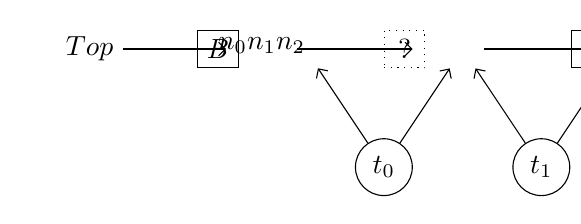
\begin{tikzpicture}[>= angle 90]
\draw (0,0) node[draw] (n0) {$B$}; \addLabel{(n0)}{$n_0$}
\draw (n0) ++ (-2,0) node (top) {$Top$}; \draw[->] (top) -- (n0);
\draw (n0) ++ (2,0) node[draw,dotted] (n1) {$\,?\,$}; \addLabel{(n1)}{$n_1$}
\draw[->] (n0) -- (n1);
\draw (n1) ++ (2,0) node[draw] (n2) {$A$}; \addLabel{(n2)}{$n_2$}
\draw[->] (n1) -- (n2);
%%% threads
\draw (n0) ++ (1,-1.5) node[draw,circle] (t0) {$t_0$};
\draw[->] (t0) -- (n0); \draw[->] (t0) -- (n1);
\draw (n1) ++ (1,-1.5) node[draw,circle] (t1) {$t_1$};
\draw[->] (t1) -- (n1); \draw[->] (t1) -- (n2);
\end{tikzpicture}
\end{center}
\caption{Illustration of a scenario from the Treiber Stack.  Nodes are
  depicted in rectangular boxes, and threads in circles.}
\label{fig:missingCommon}
\end{figure}

%%%%%

Consider the following two views
%
\begin{eqnarray*}
pre & = &  (Top(n_0), WD_B; Thread_{pop,B}(t_0, n_0, n_1), Nd_B(n_0, n_1)), \\
v & = & (Top(n_0), WD_B; Thread_{pop,B}(t_1, n_1, n_2), Nd_A(n_2, null)).
\end{eqnarray*}
%
These are depicted in Figure~\ref{fig:missingCommon}.  Both principals are
threads that are attempting to perform a pop, of nodes~$n_0$ and~$n_1$,
respectively, each having read~$B$ from that node.  Both views have an omitted
reference to node~$n_1$, depicted as dotted in the figure.  Both are possible
views of the system, but they are not consistent.

From the state $pre$, thread~$t_0$ can advance \SCALA{top} to~$n_1$,
popping~$B$, in a transition that produces
\[\mit
(Top(n_1); Thread(t_0), Nd_B(n_0, n_1)).
\]
Without condition~(c), this transition  induces a transition from~$v$ to
\[\mit
(Top(n_1); Thread_{pop,B}(t_1, n_1, n_2), Nd_A(n_2, null)).
\]
But now $t_1$ can pop~$B$ (from~$n_1$).  The watchdog will then falsely signal
an error (since it has seen~$B$ popped twice). 

Including condition~(c) will prevent this false error, since there is no state
for~$n_1$ that is consistent with the states of both~$t_0$ and~$t_1$.
Thread~$t_0$ is in a state that is consistent only with~$n_1$ holding~$A$ (it
is an invariant of the model that a $B$-node can point only to an $A$-node);
and $t_1$ is in a state that is consistent only with~$n_1$ holding~$B$.

%% Without condition~(c), the analysis finds a false error: $t_0$ pops~$B$
%% (from~$n_0$), advancing $Top$ to~$n_1$; and then $t_1$ also pops~$B$
%% (from~$n_1$).

%% In order to avoid false positives like this, we identify if the principals of
%% the two views~$pre$ and~$v$ both have a reference to the same missing
%% component, say with identity $id$.  If so, we search the set of views~$V$ to
%% try to identify a component~$c$ with identity~$id$ such that each of
%% \[
%% (pre.\fixed, \set{pre.\princ, c}) \quad\mbox{and}\quad 
%% (v.\fixed, \set{v.\princ, c}
%% \]
%% are in $V$ (recall $pre.\fixed = v.\fixed$ here). 

\begin{impNote}
This is done in \texttt{EffectOn.\linebreak[1]check\-Compatible\-Missing}.  To
fit with breadth-first search, if there is no way to instantiate the common
missing component, we store relevant information in \texttt{EffectOnStore} in
case relevant views are found subsequently.
\end{impNote}
 % induced transitions


%%%%%%%%%%%%%%%%%%%%%%%%%%%%%%%%%%%%%%%%%%%%%%%%%%%%%%%

\subsection{Correctness}

Formalise procedure.

\begin{lemma}
Let $V$ be a set of views.  Every abstract transition from~$V$ is generated by
the procedure in Definition~\ref{???}.
\end{lemma}

\begin{proof}
Consider an abstract transition
\[
\gamma(V) \ni s \trans{e} s' \sqge_{\V} v'.
\]
We need to show that we generate $v'$ as part of the process described above.

Let $fixed = s.\fixed$ and $fixed' = s'.\fixed$.  

Consider a corresponding extended transition $pre \trans{e} post$, i.e.~such
that: $pre.\fixed = fixed$,\, $post.\fixed = fixed'$; the principal of $pre$
and $post$ is the active component of the concrete transition; if another
component to which the principal has a reference synchronises on the
transition, then that is included in~$pre$ and $post$ (otherwise choose an
arbitrary view of the principal); and $pre$ and~$post$ also include any other
component relevant to the transition (i.e.~that synchronises on the transition
or to which the principal gains a reference).

\framebox{active fixed component}

Let $pId = v'.\princ.id$ be the identity of the principal of~$v'$, and suppose
that component has states $princ$ and $princ'$ in~$s$ and~$s'$, respectively
(so $princ \trans{e} princ'$).

\begin{enumerate}
\item First suppose that $pId$ is the active component in the concrete
  transition $s \trans{e} s'$, and so in the extended transition $pre
  \trans{e} post$.  And suppose that either (a)~no other component
  synchronises on the transition, or (b)~that another component does
  synchronise and is included in~$v'$, or (c)~that the principal gains a
  reference to another component in the transition, and that component is
  included in~$v'$.  In each case, the extended transition captures the
  relevant information, and so $v'$ can be extracted from~$post$.

\item Now suppose again that $pId$ is the active component in the concrete
  transition $s \trans{e} s'$, but that the secondary component~$c$ in~$v'$ is
  not in the corresponding extended transition (as in the previous case).
  Then necessarily $pId$ had a reference to~$c$ in~$s$, and $c$ did not change
  state in the transition.  Let $v = (fixed, \set{princ, c})$.  Then the
  transition $v \trans{} v'$ is induced, as in Definition\ref{def:induced-transition}

??????????

\end{enumerate}

\end{proof}
 % correctness
\section{Implementation}

The implementation uses the following types.
\begin{itemize}
\item $Transition = (Concretization, EventInt, Concretization)$.  The tuple
  $(pre, e, post)$ represents the extended transition $pre \trans{e} post$.
  The pre-state extends a view to include all other components synchronising
  on the transition, and all components to which a process gains a reference.
  The post-state gives the same components in their post-transition states. 

\item $TransitionTemplate = (Concretization, Concretization,\linebreak[1]
  Process\-Identity,\linebreak[1] EventInt, Boolean)$.  A transition template
  can be thought of as a transition with a ``hole'' for a component with a
  given identity to be slotted into.  The tuple $(pre, post, id, e, include)$
  represents an extended transition $pre \union \set{st} \trans{e} post \union
  \set{st'}$ for every state $st$ and $st'$ such that (1) $st$ and $st'$ have
  identity $id$; (2)~$st$ is compatible with $pre$; (3) if $include$ then $st
  \trans{e} st'$, otherwise $st = st'$.
\end{itemize}


The implementation includes the following state.
\begin{itemize}
\item $sysAbsViews: ViewSet$: all views found.

\item $transitions: TransitionSet$: the extended transitions found so far.

\item $transitionTemplates: TransitionTemplateSet$: the transition templates
  found so far. 

\item $nextNewViews: ArrayBuffer[ComponentView]$: new views found on the
  current ply, to be considered on the next ply.

\item $newTransitions: ArrayBuffer[Transition]$: new transitions found on the
  current ply.

\item $newTransitionTemplates: ArrayBuffer[TransitionTemplate]$: new
  transition templates found on the current ply.
\end{itemize}

In the first half of each ply, new views are added to $nextNewViews$; in the
secondhalf, they are added to $sysAbsViews$.  Likewise transitions and
transition templates are initially added to $newTransitions$ and
$new\-Transition\-Templates$, respectively.  This ensures that the sets are not
updated while we iterate over them.  On the next iteration, the program
iterates over the new views.

Figure~\ref{fig:impl} shows the relationship between some of the functions in
the implementation. 

\begin{figure}
\begin{center}
\small
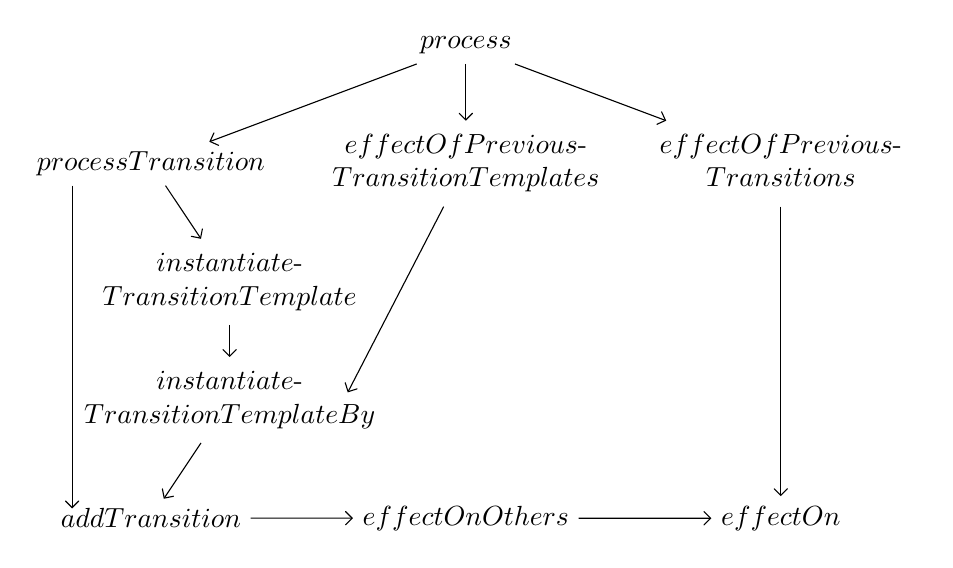
\begin{tikzpicture}[>=angle 90,yscale = 1.5]
\draw (0,0) node (process) {$process$};
\draw (process) ++ (-4,-1) node (processTransition) {$processTransition$};
%
\path[draw,->] (process) -- (processTransition);
\draw (process) ++ (0,-1) node (effectPrevTT)
   {$\begin{array}{c} effectOfPrevious\mbox{-} \\ 
       TransitionTemplates\end{array}$}; 
\path[draw,->] (process) -- (effectPrevTT);
\draw (process) ++ (4,-1) node (effectPrevTrans) 
  {$\begin{array}{c} effectOfPrevious\mbox{-} \\ Transitions\end{array}$}; 
\path[draw,->] (process) -- (effectPrevTrans);
%
\draw (processTransition) ++ (1,-1) node (instantiateTT) 
  {$\begin{array}{c} instantiate\mbox{-}\\ TransitionTemplate \end{array}$};
\path[draw,->] (processTransition) -- (instantiateTT);
%
\draw (instantiateTT) ++ (0,-1) node (instantiateTTBy)
  {$\begin{array}{c} instantiate\mbox{-}\\ TransitionTemplateBy \end{array}$};
\path[draw,->] (instantiateTT) -- (instantiateTTBy);
\path[draw,<-] (instantiateTTBy.north)++(1.5,-0.3) -- (effectPrevTT);
%
\draw (instantiateTTBy) ++ (-1,-1) node (addTransition) {$addTransition$};
\path[draw,->] (instantiateTTBy) -- (addTransition);
\draw (addTransition)++(-1,0) node (addTransitionL) {};
\path[draw,->] (processTransition.south)++(-1,0) -- (addTransitionL);
%
\draw (addTransition) ++ (4,0) node (effectOnOthers) {$effectOnOthers$};
\path[draw,->] (addTransition) -- (effectOnOthers);
%
\draw (effectOnOthers) ++ (4,0) node (effectOn) {$effectOn$}; 
\path[draw,->] (effectOnOthers) -- (effectOn);
\path[draw,->] (effectPrevTrans) -- (effectOn);
\end{tikzpicture}
\end{center}
\caption{Relationship of functions}
\label{fig:impl}
\end{figure}

The function $process(v)$ acts on a single view~$v$ found on the previous ply.
It calculates all the transitions from~$v$, together with the identities of
other components relevant to the view (if any).  It then calls
$processTransition$ on each such transition.  It also calls
$effectOfPreviousTransitions$ and $effect\-Of\-Previous\-TransitionTemplates$
on the view.

The function $processTransition(pre, e, post, ids)$ corresponds to processing
either (1)~the transition $pre \trans{e} post$, if $ids$ is empty, or
(2)~transition template $(pre, post, id, e, true)$ if $ids = \set{id}$,
i.e.~transitions with an extra component with identity~$id$ that synchronises
on~$e$.  It calculates whether the principal component gains a reference to a
component other than those in~$pre$ and~$id$.  If not and $ids$ is empty, the
transition is complete: $addTransition$ is called on it.  Otherwise, it is
added to $newTransitionTemplates$, and
$instantiate\-TransitionTemplate$ is called.

$addTransition(pre,e,post)$ adds a transition $pre \trans{e} post$ to
$new\-Transitions$, and calls $effectOnOthers$.

$effectOnOthers(pre,e,post)$ considers the effect of a new transition $pre
\trans{e} post$ on views found on previous plys.  For each such view that
matches $pre$'s fixed processes, it calls $effectOn$.

$effectOn(pre, e, post, v)$ considers the effect of a transition $pre
\trans{e} post$ on another view~$v$.  It forms all ways of combining $pre$ and
$v$, calculates the corresponding post-view for $v.\princ$, and adds it to
$nextNewViews$.

$instantiateTransitionTemplate(pre, post, id, e, inc)$ considers how to
instantiate the transition template $(pre, post,\linebreak[1] id,\linebreak[1]
e, inc)$.  For each view in $sysAbsViews$ that matches $pre$'s fixed
processes, it calls $instantiate\-Transition\-TemplateBy$.

$instantiateTransitionTemplateBy(pre, post, id, e, inc, v)$ considers how
to instantiate the transition template $(pre, post,\linebreak[1]
id,\linebreak[1] e, inc)$, so that a component of $v$ forms the extra
component with identity~$id$.  For each resulting transition, it calls
$add\-Transition$.

$effectOfPreviousTransitions(v)$ considers the effect of all previous
transitions on a view~$v$ found on the previous ply.  For each
transition in $transitions$ whose initial servers matches $v$'s servers, it
calls $effectOn$.

$effectOfPreviousTransitionTemplates(v)$ considers using a view~$v$ found on
the previous ply to instantiate the missing component in a transition
template.  For each transition template in $transitionTemplates$ whose initial
servers matches $v$'s servers, it calls $instantiateTransitionTemplateBy$.

We briefly discuss the combination of views and either transitions or
transition templates: it is important that we consider each such combination,
just once, regardless of the plys each are found or created on.  Consider a
view~$v$ found on ply~$n$, and expanded on ply~$n+1$.
%
\begin{itemize}
\item On ply~$n+1$, $v$ will be considered (in $effectOfPreviousTransitions$)
  in combination with each transition created up to ply~$n$.

\item For each transition created on ply~$n+1$ or later, its effect on~$v$
  will be considered (in $effectOnOthers$) on the ply in which the transition
  is created. 
 %% A transition from~$v$ will be considered in ply~$n+1$, and its effect
 %%  considered (in $effectOnOthers$) on all views~$v'$ found up to ply~$n$.
\end{itemize}
%
Thus the combination of a view and a transition will be treated: (1)~by the
first bullet if the transition is created on a ply no later than the view is
found; and (2)~by the second bullet if the transition is created on a ply
later than the view is found.  

Likewise
%
\begin{itemize}
\item On ply $n+1$, $v$ will be considered (in
  $effect\-Of\-Previous\-Transition\-Templates$) to create the missing
  component in each transition template created up to ply~$n$.

\item For each transition template created on ply~$n+1$ or later, its
  combination with~$v$ will be considered (in
  $instantiate\-Transition\-Template$) on the ply in which the transition
  template is created.
%% \item A transition template from~$v$ will be created in ply~$n+1$, and all
%%   ways of creating the missing component from views found up to ply~$n$ will
%%   be considered (in $instantiateTransitionTemplate$).
\end{itemize}
%
Thus the combination of a view and a transition template will be treated:
(1)~by the first bullet if the transition template is created on a ply no
later than the view is found; and (2)~by the second bullet if the transition
template is created on a ply later than the view is found.

%%%%%%%%%%%%%%%%%%%%%%%%%%%%%%%%%%%%%%%%%%%%%%%%%%%%%%%

\subsection{instantiateTransitiontemplateBy}

$instantiateTransitionTemplateBy(pre, post, id, e, inc, v)$ considers how
to instantiate the transition template $(pre, post,\linebreak[1]
id,\linebreak[1] e, inc)$, so that a component of $v$ forms the extra
component with identity~$id$.  For each resulting transition, it calls
$add\-Transition$.


The function $consistentStates(pre, id, e, inc, v)$ considers how to rename
$v$ to potentially produce the extra component of the transition template
$(pre, post,\linebreak[1] id,\linebreak[1] e, inc)$.  More precisely, it finds
all ways of renaming~$v$ to obtain a view~$v'$ so that (1) a component of~$v'$
has identity~$id$, (2)~$v'$ and~$pre$ agree on common components, and (3)~if
$inc$ then $v'$ can perform~$e$.  For each, it returns the renamed component
with identity id, and the next states. 

For each such extra component~$st$,\, $isExtendable(pre, st)$ tests whether
$st$ is consistent with $pre$, in the sense that for each component $c$ of
$pre \union st$, the current set of views contains a view with $c$ as
principal component and agreeing on common processes (modulo renaming).

$compatibleWith(servers, components, st)$ tests whether there is an existing
view with $st$ as principal component that agrees with $servers$ and
$components$ on common processes. 

$containsReferencingView(pre, st, j)$ assumes that $pre.components(j)$ has a
reference to $st$.  If tests whether there is a view with $pre.components(j)$
as principal component, containing $st$, and otherwise compatible with~$pre$
(modulo renaming).

*** If the views that ensure consistency are found later, do we get all
instantiations?  I think so.  The last relevant view will include the state we
want. 

%\newpage
\section{Calculating induced transitions with symmetry reduction}
\label{sec:induced-symmetry}

In this section, we consider consider how to calculate the transition induced
by a transition $pre \trans{e} post$ on a view~$v$, given that both are in
normal form and represent all members of their equivalence classes.  
%
Following Definition~\ref{def:induced-transition}, in principle, we need to
find all ways of renaming parameters of~$v$ and~$pre$ to produce views that
are accordant.  However, if two different renamings would produce equivalent
post-views, it is enough to consider just one of them.  It is therefore enough
to keep the parameters of $pre$ fixed, and to rename the parameters of~$v$.
Each renaming can be defined by an renaming~$\pi$ over the parameters of~$v$.
That is, we consider renamings~$\pi$ such that $\pi(v)$ and~$pre$ are
accordant, and consider the effect of the transition on~$\pi(v)$.
%
Below, we restrict the range of such renamings further, while ensuring we
produce a representative of each equivalence class of resulting post-views.


%% We start by considering full views; in Section~\ref{sec:effectOn-restricted}
%% we consider restricted views.

%%%%%%%%%%%%%%%%%%%%%%%%%%%%%%%%%%%%%%%%%%%%%%%%%%%%%%%

%\subsection{Full views} 
%\label{ssec:effectOn-full}

Recall that in order to be accordant, if $\pi(v)$ and $pre$ each have a
component with the same identity, then those components must be equal.  We say
that the renaming has \emph{unified} these components.
%
\begin{definition}
Let $v$ and $pre$ be in normal form.  Then renaming function~$\pi$ over the
parameters of~$v$ is a \emph{unification function} if $\pi(v)$ and $pre$ are
accordant.
%
If $c$ is a component of~$v$, $c'$ is a component of~$pre$, and $\pi(c) = c'$,
we say that $c$ and~$c'$ are \emph{unified}.
\end{definition}
%
Of course, it is possible to unify two components only if they have the same
control state. 

Recall that if $\pi(v)$ and~$pre$ are accordant, then their fixed processes
are equal.  The following lemma follows from the way we have defined normal
forms. 
%% But $v$ and $pre$ are stored in normal form, so this will be the
%% case only if the fixed processes of $v$ and~$pre$ are equal, and
%% $\pi$ is be the identity function on all parameters of those fixed
%% processes.  
%
\begin{lemma}
If $v$ and~$pre$ are both in normal form, and $\pi(v)$ and~$pre$ are
accordant, then $v.\fixed = pre.\fixed$ and $\pi$ is the identity over the
parameters of~$v.\fixed$.
\end{lemma}

%%%%%

\begin{example}
We use a running example to illustrate the technique.  Consider
\begin{eqnarray*}
pre & = &
   (fixed(N_0); Th(T_0, N_1, N_2), Nd_A(N_1, N_3), Nd_B(N_2, N_0, N_4)), 
\\
post & = & 
  (fixed'(N_5); Th'(T_0, N_1, N_2), Nd_C(N_1, N_2, N_3), Nd_B(N_2, N_0, N_4)) ,
\\
v & = & 
  (fixed(N_0); Nd_A(N_1, N_2), Nd_B(N_2, N_0, N_3)).
\end{eqnarray*}
%
$pre$ and~$v$ have fixed processes in the same states, so there is the
potential to produce a renaming~$\pi(v)$ accordant with~$pre$.  We start with
the partial renaming function $\pi = \set{N_0 \mapsto N_0}$, the identity over
the parameters of the fixed processes.

It is worth noting that the identifiers $N_1$, $N_2$ and~$N_3$ that appear in
both~$pre$ and~$v$ might represent different parameters, since each substate
is just a representative of its equivalence class.  The fact that the same
identifiers appear in each substate is just an artefact of the way we produce
normal forms.
\end{example}

%%%%%

In general, any subset of the components of~$v$ might be unified with
components of~$pre$ (including no unifications).  For each potential choice of
which components to unify, we construct the minimal renaming function that
extends the identity function over the parameters of the fixed processes so as
to rename the parameters of each unified component of~$v$ to the parameters of
the corresponding component of~$pre$.  We call the resulting function a
\emph{partial unification function}.  However, some such choices of
unifications might prove impossible, if no such function exists.
%
\begin{definition}
Let $v$ and $pre$ be in normal form with $v.\fixed = pre.\fixed$.  Then a
partial renaming function~$\pi$ is a \emph{partial unification function} if
\begin{itemize}
\item $\pi$ is the identity function over the parameters of $v.\fixed$;

\item $\pi$ is defined over the parameters of a subset of the components
  of~$v$, mapping each such component to unify it with a component of $pre$;

\item $\pi$ is undefined over all parameters not included under the previous
  two points.
\end{itemize}
\end{definition}


%%%%%

\begin{example}
We continue with the running example.  Unifying the two $Nd_A$ processes
gives the partial unification function
%
\begin{eqnarray*}
\pi_1 & = & \set{N_0 \mapsto N_0, N_1 \mapsto N_1, N_2 \mapsto N_3}.
\end{eqnarray*}
%
Alternatively, unifying the two $Nd_B$ processes gives
\begin{eqnarray*}
\pi_2 & = & \set{N_0 \mapsto N_0, N_2 \mapsto N_2, N_3 \mapsto N_4}.
\end{eqnarray*}
It is not possible to unify both pairs simultaneously, since $N_2$ cannot be
mapped consistently.  In addition, the renaming~$\pi$ corresponds to unifying
no components.
\end{example}

We now need to extend each such renaming function in a consistent way.  The
following definition describes what that means.
%
\begin{definition}
\label{def:consistent-extension}
Let $pre \trans{e} post$ be an extended transition, and $v$ be a view, both in
normal form, with $v.\fixed = pre.\fixed$.
%
Consider a partial unification function~$\pi$.  We define an extension~$\pi'$
of~$\pi$ to be a \emph{consistent extension} if (a)~the renaming~$\pi'$ is
injective and defined over all parameters of~$v$; and (b)~whenever a
component~$c$ in~$v$ is not unified with any component of~$pre$, the identity
of~$c$ is not mapped to an identity of a component~$c'$ in~$pre$ (since that
would require unifying~$c$ and~$c'$).
\end{definition}

%%%%%

The following lemma follows directly from the definitions.
%
\begin{lemma}
Let $pre \trans{e} post$ be an extended transition, and $v$ be a view, both in
normal form, with $v.\fixed = pre.\fixed$.  Then every unification
function~$\pi$ is a consistent extension of a partial unification function,
and vice versa.
\end{lemma}

In principal, then, we need to consider all consistent extensions of all
partial unification functions.  However, many different consistent extensions
will end up producing the same new view, up to equivalence, so it will be
enough to build only representative renamings.  Recall
(Definition~\ref{def:induced-transition}) that when we build an induced
transition, the state of each component in the new view is: (1)~the state
from~$post$ for components in the transition; or (2)~the state from~$v$ for
other components.  The unifications already tell us the states in case~(1).
In case~(2), each parameter in the component might or might not be the same as
a parameter taken from $post$.  We need to find all ways of renaming
parameters in such components to give distinct new views, up to equivalence.
The following definition captures the required consistent extensions; we
verify this fact as Proposition~\ref{prop:unifying-renaming}.

%%%%%

\begin{definition}
\label{def:representative-consistent-extension}
Consider an extended transition~$pre \trans{e} post$, a view~$v$, and a
partial unification function~$\pi$.  We define a consistent extension~$\pi'$
of~$\pi$ to be a \emph{representative consistent extension} if for every
parameter~$x$ in~$v$ but not in the domain of~$\pi$,\, $\pi'(x)$ is one of the
following:
%
\begin{enumerate}
\item\label{clause:remap-1} a parameter of $post.\fixed$; 

\item\label{clause:remap-2} a parameter of the state in~$post$ of a unified
  component;

\item\label{clause:remap-3} if the principal of~$v$ is unified with a
  component~$c$, and $c$~gains a reference to a component with identity~$id$,
  then a parameter of the state in~$post$ of~$id$ (note that $pre$ and $post$
  must contain a component with identity~$id$, by
  clause~\ref{assump:secondary-cpts-new-refs} of Assumption~\ref{assump}); or

\item\label{clause:remap-4} a minimal fresh parameter, i.e.~a parameter
  different from those in~$pre$ and~$post$, and in each case choosing (in the
  order in which those parameters~$x$ appear in~$v$) the minimal such value
  that hasn't been used previously. 
\end{enumerate}
%
%% Further, under case~\ref{clause:remap-4}, \emph{minimal} fresh parameters are
%% chosen for each such~$x$, in the order in which those parameters~$x$ appear
%% in~$v$ (i.e.~in each case choosing the smallest fresh parameter not already
%% used).
%
Note that these are subject to the conditions~(a) and~(b) of
Definition~\ref{def:consistent-extension}. 
%% These are all subject to two provisos: (a)~that the renaming remains
%% injective; and (b)~a parameter that is the identity of a component~$c$ in~$v$
%% that is not unified with any component of~$pre$ cannot be mapped to an
%% identity of a component in~$pre$ (since that would require unifying~$c$).
\end{definition}
%
%% When a parameter is mapped to a fresh parameter, all choices of the fresh
%% parameter give equivalent post-states.  Hence it is enough to make the choice
%% in one way: we pick the minimal fresh parameter each time. 


%%%%%

\begin{example}
We continue the running example, considering just the unification
corresponding to~$\pi_1$.  Consider what values~$N_3$ can be mapped to.  By
clause~\ref{clause:remap-1}, it can be mapped to~$N_5$.  By
clause~\ref{clause:remap-2}, it can be mapped to~$N_2$.  By
clause~\ref{clause:remap-3}, it can be mapped to~$N_4$ (from the post-state of
the $Nd_B$ process).  Finally, by clause~\ref{clause:remap-4}, it can be
mapped to the minimal fresh value, namely~$N_6$.
%
This then produces four renamings:
\[
\pi_X = \set{N_0 \mapsto N_0, N_1 \mapsto N_1, N_2 \mapsto N_3, N_3 \mapsto X},
\quad \mbox{for $X = N_2, N_4, N_5, N_6$}.
\]
For each such renaming~$\pi_X$,\, $v$ gets remapped to a view of the form
\[
(fixed(N_0); Nd_A(N_1, N_3), Nd_B(N_3, N_0, X)).
\]
The $fixed$ and $Nd_A$ processes evolve under the transition \( pre
\trans{} post \), and the latter gains a reference to~$N_2$ in
$post$.  This produces the four views
\[
(fixed'(N_5); Nd_C(N_1, N_2, N_3), Nd_B(N_2, N_0, N_4), Nd_B(N_3, N_0, X)).
\]
Finally, these views need to be reduced to normal form.  Note that the four
normal forms are distinct.
\end{example}

%%%%%

The following proposition shows that considering representative consistent
extensions is enough to produce all induced transitions, up to equivalence. 
%
\begin{prop}
\label{prop:unifying-renaming}
Consider an extended transition $pre \trans{e} post$ and a view~$v$, both in
normal form, with $v.\fixed = pre.\fixed$.  Consider also a partial
unification function~$\pi$.
%
Let $\pi'$ be a consistent extension of~$\pi$, and
let $v'$ be the view produced by Definition~\ref{def:induced-transition}
considering the effect of $pre \trans{e} post$ on~$\pi'(v)$.  
%
Then there is a representative consistent extension~$\pi''$ of~$\pi$, such
that, letting $v''$ be the view produced by
Definition~\ref{def:induced-transition} considering the effect of $pre
\trans{e} post$ on~$\pi''(v)$, we have $v'' \equiv v'$.
\end{prop}

%%%%%%

\begin{proof}
Let $pre$, $post$, $v$, $\pi$, $\pi'$ and~$v'$ be as in the statement of the
lemma.  We describe how to construct the renaming~$\pi''$, and a
renaming~$\hat\pi$ such that $\pi' = \hat\pi \circ \pi''$.  This will imply
that $\hat\pi(v'') = v'$.  The following figure illustrates (and acts as an
aide-m\'emoire).
%
\begin{center}
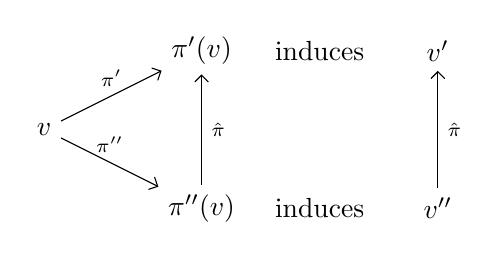
\begin{tikzpicture}[>= angle 90]
\draw (0,0) node (v) {$v$};
%
\draw (2,1) node (pi'v) {$\pi'(v)$};
\path[draw, ->] (v) -- node[above]{\scriptsize $\pi'$} (pi'v);
%
\draw (2,-1) node (pi''v) {$\pi''(v)$};
\path[draw, ->] (v) -- node[above]{\scriptsize $\pi''$} (pi''v);
\path[draw, ->] (pi''v) -- node[right]{\scriptsize $\hat\pi$} (pi'v);
%
\draw (pi'v)++(1.5,0) node (induces1) {induces};
\draw (induces1)++(1.5,0) node (v') {$v'$};
%
\draw (pi''v)++(1.5,0) node (induces2) {induces};
\draw (induces2)++(1.5,0) node (v'') {$v''$};
\path[draw, ->] (v'') -- node[right]{\scriptsize $\hat\pi$} (v');
\end{tikzpicture}
\end{center}
%
In fact, $\hat\pi$ will be the identity over all parameters except for fresh
parameters chosen under clause~\ref{clause:remap-4} of
Definition~\ref{def:representative-consistent-extension}.

We define $\pi''$ as an extension of~$\pi$.  This implies that $\pi''$
and~$\pi'$ agree on values in the domain of~$\pi$, and unify the same
components.  For all values~$y$ in the range of~$\pi$, we define $\hat\pi(y) =
y$. 

Recall that $v'.\fixed = v''.\fixed = post.\fixed$; each component of~$v'$ is
taken from~$post$ if the corresponding component of~$\pi'(v)$ is in~$pre$, and
otherwise is taken from~$\pi'(v)$; and each component of~$v''$ is taken
from~$post$ if the corresponding component of~$\pi''(v)$ is in~$pre$, and
otherwise is taken from~$\pi''(v)$.  We arrange for~$v'$ and~$v''$ to take the
same components from~$post$.

%% For each parameter~$x$ of~$v.\fixed$, we define $\pi''(x) = x$.  This means
%% $\pi''(v).\fixed = pre.fixed$.  And we define $\hat\pi(x) = x$. 

For each parameter~$x$ of~$v$ such that $y = \pi'(x)$ is a parameter of
$post.\fixed$, we define $\pi''(x) = y$, and $\hat\pi(y) = y$.  Note that each
such value~$y$ is included under case~\ref{clause:remap-1} of
Definition~\ref{def:representative-consistent-extension}.  This ensures
that~$\pi''(v)$ and~$\pi'(v)$ agree on all such~$y$; and hence~$v'$ and~$v''$
agree on all such~$y$.  Note that this is a consistent extension of~$\pi$,
because~$\pi'$ is a consistent extension of~$\pi$.  

For each parameter~$x$ such that $y = \pi'(x)$ is a parameter of a component
of~$v'$ taken from~$post$, we again define $\pi''(x) = y$, and $\hat\pi(y) =
y$.  Note that each such value $y$ is included under
case~\ref{clause:remap-2} or \ref{clause:remap-3} of
Definition~\ref{def:representative-consistent-extension}.  This ensures
that~$\pi''(v)$ and~$\pi'(v)$ agree on all such~$y$; and hence~$v'$ and~$v''$
agree on all such~$y$; in particular, they include the same components taken
from~$post$.  Again note that this is a consistent extension of~$\pi$,
because~$\pi'$ is a consistent extension of~$\pi$. 

Finally, each other parameter~$y$ in~$v'$ must necessarily be in a component
taken from~$\pi'(v)$.  Suppose the parameter is $\pi'(x)$, and $x$ is not in
the domain of~$\pi$.  We define $\pi''(x)$ to be the minimal fresh
parameter~$z$, chosen as in
Definition~\ref{def:representative-consistent-extension}; and we let
$\hat\pi(z) = y$.  This ensures that $v''$ uses~$z$ wherever $v'$ uses~$y$.
Also note that this is a consistent extension of~$\pi$, by construction.
\end{proof}

%%%%%

\begin{impNote}
\texttt{Unification.combine} produces the remapped version of~$v$, together
with information about the unifications.  If uses \texttt{allUnifs} to find
all choices of unification and corresponding renaming function~$\pi$.  Then
\texttt{extendUnif} extends this, and produces the remapped state.

\texttt{EffectOn.apply} produces the corresponding post-views.
\end{impNote}

%%%%%

\subsection{Optimisations} 


%%%%%

\begin{opt}
Recall Optimisation~\ref{opt:avoid-induced}.  
\begin{itemize}
\item For case~\ref{case:avoid-induced-1}, we avoid unifying the principal
  of~$v$ with the principal of~$pre$.

\item For case~\ref{case:avoid-induced-2}, if $pre.\fixed = post.\fixed$ we
  require that at least one component of~$v$ unifies with a component that
  changes state.

\item For case~\ref{case:avoid-induced-3}, we store a record of pairs
  $(v, post.\fixed)$ for which we have considered the effect of a transition
  $pre \trans{e} post$ on~$v$ for which $pre.\fixed \ne post.\fixed$,\,
  %% $unifs$ describes which components of~$v$ unify with which components
  %% of~$pre$ (
  and $v$
  unifies with no component.
%
  If subsequently we consider a similar case ---that is, the same
  $post.\fixed$ and~$v$, and no unifications--- we identify that it will not
  produce any new views, and so avoid the construction.
\end{itemize}
\end{opt}


\begin{impNote}
Done in isSufficientUnif. 
\end{impNote}

\begin{improve}
The third case is not quite the same as in
Optimisation~\ref{opt:avoid-induced}.  There we included cases where $pre$
and~$v$ shared a component that did not change state.  An obvious attempt to
implement this goes wrong: if there are two cases with the same $post.\fixed$
and~$v$, that include unifications of \emph{different} components that do not
change state, they might give different new views (with the unified components
having different parameters in $post.\fixed$).
%
For example
\begin{eqnarray*}
pre & = & (fixed; Th_1(T_0,N_0), Nd_A(N_0,N_1)) \\
post & = & (fixed'(N_1); Th_1'(T_0), Nd_A(N_0,N_1)) \\
v & = & (fixed; Th_v(T_0,N_0), Nd_A(N_0,N_1))
\end{eqnarray*}
unifying the two $Nd_A$ processes, with remapping $\set{T_0 \mapsto T_1, N_0
  \mapsto N_0,\linebreak[1] {N_1 \mapsto N_1}}$, induces
\[
(fixed'(N_1); Th_v(T_1,N_0), Nd_A(N_0,N_1) \equiv
(fixed'(N_0); Th_v(T_0,N_1), Nd_A(N_1,N_0)).
\]
But with 
\begin{eqnarray*}
pre' & = & (fixed; Th_2(T_0,N_0,N_1), Nd_A(N_0,N_2), Nd_N(N_1,Null)) \\
post' & = & (fixed'(N_1); Th_2'(T_0), Nd_A(N_0,N_2), Nd_N(N_1,Null))
\end{eqnarray*}
unifying the two $Nd_A$ processes, with remapping $\set{T_0 \mapsto T_1, N_0
  \mapsto N_0,\linebreak[1] {N_1 \mapsto N_2}}$, induces a transition to
\[\mit
(fixed'(N_1); Th_v(T_1,N_0), Nd_A(N_0,N_2)) \equiv
  (fixed'(N_0); Th_v(T_0,N_1), Nd_A(N_1, N_2)).
\]


If we have two cases concerning the same $post.\fixed$, $v$, and component~$c$
of~$v$ that unifies and doesn't change state, and $c$ unifies respectively
with~$c_1$ and~$c_2$ which differ only on parameters not in $post.\fixed$,
then it is enough to consider just one such case.  In the above example, we
had $c_1 = Nd_A(N_0,N_1)$,\, $c_2 = Nd_A(N_0,N_2)$ which differ on~$N_1$. 

\framebox{Do this.}  For the components, it's enough to store the list of
parameters shared with $post.\fixed$ and their indices. 
\end{improve}

 
%%%%%%%%%%%%%%%%%%%%

\begin{opt}
If the principal of~$v$ is unified with a component of~$pre$, and loses a
reference to a component~$c$, then all renamings of~$c$ produce the same final
view.  Thus it is enough to consider a single renaming, say the renaming that
agrees with the renaming within other components, but otherwise maps to fresh
parameters.  There is no need to explicitly construct the renaming of~$c$.  
%
\framebox{Consider this.}

This won't work with singleRef, however, because of cross references or
missing references. 
\end{opt}

%%%%%

\begin{improve} 
If the principal and another component~$c$ of~$v$ are both unified with
components of $pre$, and the principal of~$v$ loses the reference to~$c$ in
the transition, then for case~\ref{clause:remap-2} of
Definition~\ref{def:representative-consistent-extension}, we can ignore
parameters of~$c$.  This is only relevant for renaming of some third
component.
%
This might be useful when a node has a reference to the thread, but loses
that reference.
\end{improve}


%%%%%%%%%%%%%%%%%%%%%%%%%%%%%%%%%%%%%%%%%%%%%%%%%%%%%%%


\end{document}
